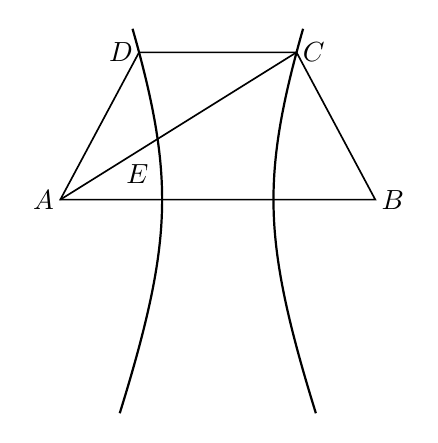
\begin{tikzpicture}[x=1cm,y=1cm,font=\normalsize,line width=.6pt]
% coordinate frame: A=(-2,0), B=(2,0), C=(1,1.8708), D=(-1,1.8708)
% hyperbola x^2/0.5-y^2/3.5=1, i.e. x=+-sqrt(0.5*(1+y^2/3.5))
\coordinate (A) at (-2,0);
\coordinate (B) at (2,0);
\coordinate (C) at (1.0000000000,1.8708286934);
\coordinate (D) at (-1.0000000000,1.8708286934);
\coordinate (E) at (-0.7647058824,0.7703412267);
% trapezoid
\draw (A) -- (B) -- (C) -- (D) -- cycle;

% diagonal A-C with E on it
\draw (A) -- (C);
% hyperbola branches from formula (not freehand)


% labels clear of strokes
\node[inner sep=2pt,anchor=east] at ([xshift=0pt]A) {$A$};
\node[inner sep=2pt,anchor=west] at ([xshift=0pt]B) {$B$};
\node[inner sep=2pt,anchor=west] at ([xshift=0pt]C) {$C$};
\node[inner sep=2pt,anchor=east] at ([xshift=0pt]D) {$D$};
\node[inner sep=2pt,anchor=north east,xshift=-1pt,yshift=-7pt] at ([xshift=0pt,yshift=0pt]E) {$E$};
\draw[line width=.8pt] plot[variable=\t,domain=-2.7127016054111075:2.170161284328886,samples=120] ({sqrt(0.5*(1+\t*\t/3.5))},\t);
\draw[line width=.8pt] plot[variable=\t,domain=-2.7127016054111075:2.170161284328886,samples=120] ({-sqrt(0.5*(1+\t*\t/3.5))},\t);
\end{tikzpicture}
